% -----------------------------------------------------------------
% Section 5.4 Extension: Robustness paragraph
%   Insert after the existing "Robustness to normalisation choices"
%   paragraph in Section 5.4.
%   Requires: figures/fig9_robustness_yield_curve.pdf
% -----------------------------------------------------------------

\paragraph{Robustness to source composition.}
The structural fragmentation signal is robust to source exclusion:
removing any single source yields $z$-scores ranging from $-7.8$ to
$-5.2$ (all ${p < 0.001}$), except when Open LLM Leaderboard~v2 is
excluded---which reduces the dataset to 2{,}541 records and the
expected collision count to just~2.7, producing 5~observed collisions
and $z = 1.4$ (not significant). This exception is expected: OLv2
contributes 91\% of records and participates in 6~of~16 collision
pairs; without it, the ecosystem is too small for the null model to
predict more than~${\sim}3$ collisions.
Under strict normalisation (6~observed collisions), the $z$-score is
$-7.6$---more extreme than the default ($z = -6.4$), confirming that
conservative normalisation \emph{strengthens} rather than weakens the
fragmentation finding.
Figure~\ref{fig:yield} shows that the gap between observed and
expected collisions is present from $k = 3$ sources onward and widens
monotonically---ruling out small-sample artefacts.

\begin{figure}[t]
\centering
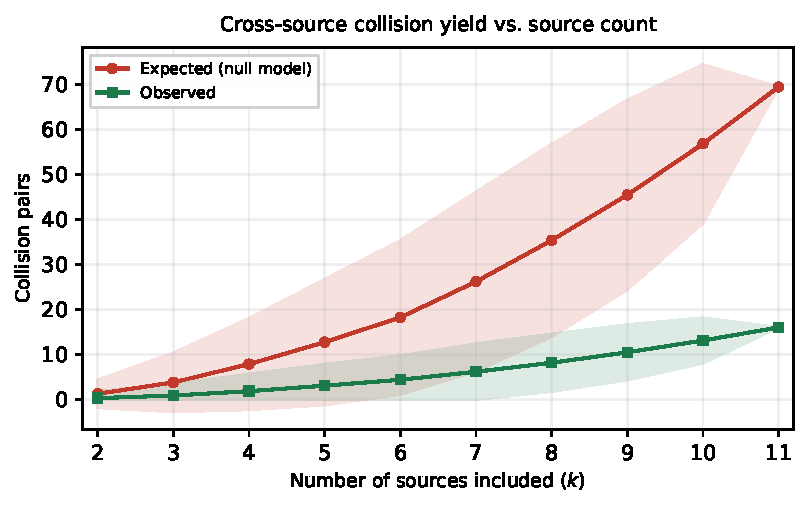
\includegraphics[width=\columnwidth]{figures/fig9_robustness_yield_curve.pdf}
\caption{Collision yield curve. For each source-subset size~$k$
(2--11), we plot the mean observed collision count (green) and the
mean expected count under the null model (red), with $\pm 1$~SD
bands. The observed curve lies below the expected curve at every~$k$,
confirming that structural fragmentation is a systemic property of the
evaluation ecosystem rather than a small-sample artefact.}
\label{fig:yield}
\end{figure}
